\documentclass[11pt]{article}

\newcommand{\cnum}{CM146}
\newcommand{\ced}{Fall 2017}
\newcommand{\ctitle}[3]{\title{\vspace{-0.5in}\cnum, \ced\\Problem Set #1: #2\\Due #3}}
\usepackage{enumitem}
\usepackage{graphicx}
\newcommand{\solution}[1]{{{\color{blue}{\bf Solution:} {#1}}}}
\usepackage[usenames,dvipsnames,svgnames,table,hyperref]{xcolor}

\renewcommand*{\theenumi}{\alph{enumi}}
\renewcommand*\labelenumi{(\theenumi)}
\renewcommand*{\theenumii}{\roman{enumii}}
\renewcommand*\labelenumii{\theenumii.}
\graphicspath{{images/}}

\begin{document}
\ctitle{1}{Atibhav Mittal (ID:804598987)}{Jan 30, 2017}
\author{}
\date{}
\maketitle
\vspace{-0.75in}

\section{Problem 1}
\begin{enumerate}
\item Problem 1a

\solution{} \newline
Without splitting the data even once, we have two possible cases $y=1$ or $y = 0$

If we predict $y=1$ always, number of mistakes = $2^{n-3}$
If we predict $y=0$ always, number of mistakes = $2^n - 2^{n-3} = 7 \cdot 2^{n-3}$

Hence, the best 1-leaf decision tree will make at least $2^{n-3}$ mistakes

\item Problem 1b

\solution{} \newline
No there is no such split that reduces the number of mistakes by at least 1. 
Since our target function is $X_{1} \lor X_{2} \lor X_{3}$, the best case would be to 
have the first internal node, split based on one of these indicators. 
Because of symmetry, it doesn't matter which indicator we choose. 
So let's say the first decision node split based on $X_{1}$

If $X_{1} = 1$, we predict $y=1$
If $X_{1} = 0$, we can either predict 0 or 1.
In case we predict y = 1, number of mistakes = $2^{n-3}$
In case we predict y = 0, number of mistakes = $2^{n-1} - 2^{n-3} = 3 \cdot 2 ^{n-3}$

Hence, the minimum number of mistakes we'll make is still $2^{n-3}$

\item Problem 1c
\solution{} 
$$
Entropy(S) = - \left( \frac{2^n - 2^{n-3}}{2^n}\right) \log \left( \frac{2^n - 2^{n-3}}{2^n}\right) - \left( \frac{2^{n-3}}{2^n} \right) \log \left( \frac{2^{n-3}}{2^n} \right)
$$
$$
Entropy(S) = \frac{4.4}{8} = 0.55
$$

\item Problem 1d
\solution{}
Yes, a split based on $X_{1}$ would reduce the entropy.

Entropy($X_{1} = 1$) $ = - 0 \log(0) - 1 \log(1) = 0$ \newline
Entropy($X_{1} = 0$) $ = - \left( \frac{2^{n-1} - 2^{n-3}}{2^{n-1}}\right) \log \left( \frac{2^{n-1} - 2^{n-3}}{2^{n-1}}\right) - \left( \frac{2^{n-3}}{2^{n-1}} \right) \log \left( \frac{2^{n-3}}{2^{n-1}} \right)$ \newline
Entropy($X_{1} = 0$) $ = 0.812$

Conditional Entropy = $\frac{2^{n-1}}{2^n} (0) + \frac{2^{n-1}}{2^n} (0.812) = 0.406$ \newline

Hence, this split reduces the entropy by $0.55 - 0.406 = 0.144$
\end{enumerate}

\newpage
\section{Problem 2}

\solution{} \newline
Entropy Before the split = $B \left(\frac{p}{p+n} \right)$
$$
 = - \left(\frac{p}{p+n} \right) \log \left(\frac{p}{p+n}\right) - \left(\frac{n}{p+n} \right) \log \left(\frac{n}{p+n}\right)
$$


Entropy After the Split = $ \sum\limits_{i=1}^{k} \frac{p_{k} + n_{k}}{p + n}$ Entropy$(S_{k})$ \newline
Entropy After the Split = $\frac{p_{k} + n_{k}}{p + n}$ ( Entropy $(S_k) ) \sum\limits_{i=1}^{k} 1$ \newline
Entropy After the Split = $ k \cdot \frac{p_k + n_k}{p + n}$ ( Entropy $(S_k)$) \newline
Entropy After the Split = $ \frac{k \cdot (p_k + n_k)}{p + n}$ ( Entropy $(S_k)$) $ = \frac{p+n}{p+n}$ ( Entropy $(S_k)$) 
\bigbreak
Entropy After the Split = Entropy $(S_k)$
\bigbreak
Entropy($S_{k}$) = $ - \left( \frac{p_k}{p_k + n_k} \right) \log \left( \frac{p_k}{p_k + n_k} \right) - \left( \frac{n_k}{p_k + n_k} \right) \log \left( \frac{n_k}{p_k + n_k} \right)$
\bigbreak
The fraction $\frac{p_k}{p_k + n_k} = \frac{p}{p + n}$ (Since $p = kp_k$ and $n = kn_k$) \newline
Entropy($S_{k}$) = $
 = - \left(\frac{p}{p+n} \right) \log \left(\frac{p}{p+n}\right) - \left(\frac{n}{p+n} \right) \log \left(\frac{n}{p+n}\right) $ 
\bigbreak
This is equal to the Entropy Before the split. 
\bigbreak
Information Gain = $Entropy_{before} - Entropy_{after} = 0$ \newline
Hence, proved
\newpage

\section{Problem 3}
\begin{enumerate}
\item 
\solution{} \newline
The value of k = 1 minimizes the training error.
Since every point is a neighbor of itself, the training error = 0

\item
\solution{} \newline
Using large values of k might be bad because there is no clear clustering of the positive 
and negative points, i.e. they are mixed well. Because of this, the negative points towards
the bottom-right of the graph will be classified as positive incorrectly, and same with the
negative points at the top left \newline
Using really small values might be bad because
for instance, k = 1, each point is classified as itself, which leads to overfitting.
Furthermore other smaller values of k such as 2 or 3 will also increase the training error
as the points aren't clustered together.

\item 
\solution{} \newline
k = 5 minimizes the leave-one-out cross-validation error \newline
The error in that case would be the 4 points that are in the top left
or the bottom right.

\end{enumerate}

\newpage
\section{Problem 4}
\solution{Solution to problem 4}

\begin{enumerate}
\item 
\begin{enumerate}
\item Age: The survived category based on age is as expected since the 
		number of people aged 20-40 will be higher than the rest. However,
		we can see that a larger percentage of infants and old people survived.	
\item Embarked: The graph shows that majority of the people boarded the ship
		at the port encoded as $2$. A larger percentage of people who boarded the
		ship at port $0$ survived, so it is possible that people boarding the 
		ship at port $0$ had a better chance for survival. But for port $0$ and
		port $1$, the trends are as expected where majority of the people did not
		survive.
\item Fare: This graph shows that people who paid higher fares had a better
		chance of surviving. It also shows that a majority of the people paid
		lower fares, so the inference that higher fare corresponds to better chance
		of survival may be incorrect.
\item PClass: The PClass graph shows that people who were in a better class of the
		ship had a better chance of survival. This could be due to earlier evacuation
		of people in first/second class compared to people in the third class.
\item Parch: This graph shows that most of the people didn't travel with their parents/children
		Those who did, had a better chance of survival because they were probably 
		let off the ship first.
\item Sex: The histogram generated shows that a majority of the female passengers
		survived. Hence, a female on Titanic would have a better chance of survival
\item Sibsp: The graph shows that the number of people traveling with their siblings/spouses
		is pretty low and people traveling with only 1 sibling/spouse had a better
		chance of survival.
\end{enumerate}
\newpage
\item 
\solution{}
\newline
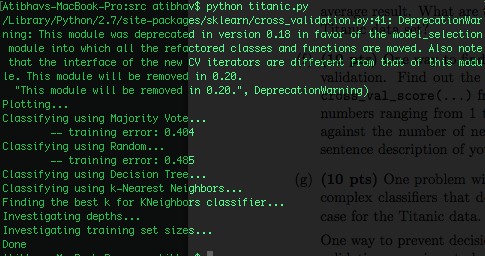
\includegraphics[scale=0.6]{4b.png}

\item
\solution{} \newline
The training error using a DecisionTreeClassifier is: $0.014$

\item
\solution{}
\begin{enumerate}
\item Training Error (k = 3): 0.167
\item Training Error (k = 5): 0.201
\item Training Error (k = 7): 0.240
\end{enumerate}

\item
\solution{}
\begin{center}
\begin{tabular}{| c | c | c |}
\hline
Classifier & Train Error & Test Error \\
\hline
Majority Vote Classifier & 0.404 & 0.407 \\
\hline
Random Classifier & 0.489 & 0.486 \\
\hline
Decision Tree Classifier & 0.012 & 0.241 \\
\hline
K-Neighbors Classifier & 0.213 & 0.315 \\
\hline

\end{tabular}
\end{center}
\newpage
\item
\solution{} \newline
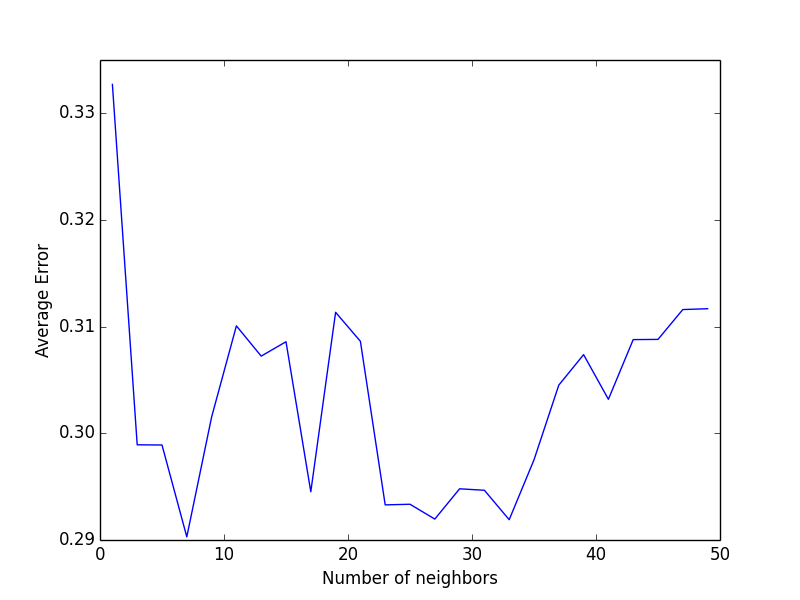
\includegraphics[scale=0.6]{4f.png}
From the above graph, the validation error is minimum at k = 7\newline
We can see that initially for low values of k, the error is high as expected. 
At k = 7, this error goes to its minimum and then increases after ( k $>$ 7) due to overfitting.
\newpage
\item
\solution{} \newline
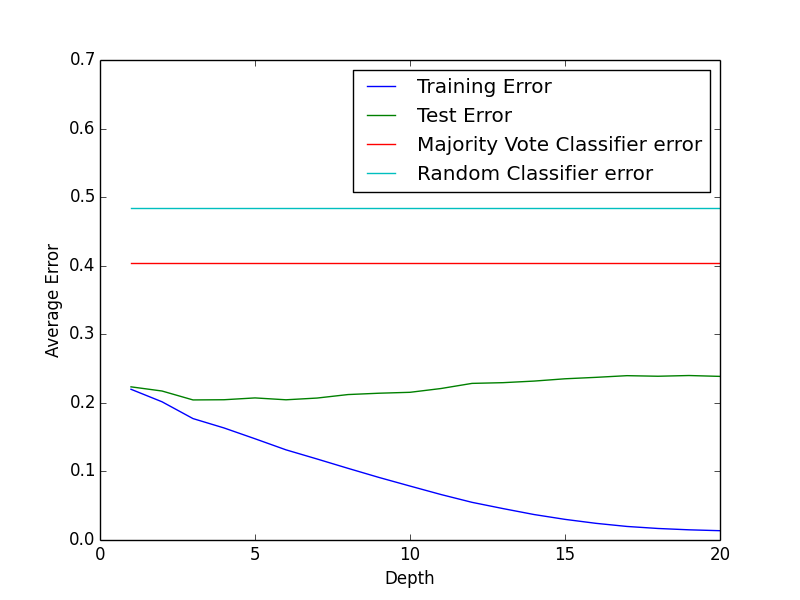
\includegraphics[scale=0.6]{4g.png}
From the above graph we can see that the best depth limit to avoid overfitting is 6
that the test error is at its lowest. As depth limit $\rightarrow$ 10, the training error goes down but
the test error increases. This is due to overfitting. 
\newpage
\item
\solution{} \newline
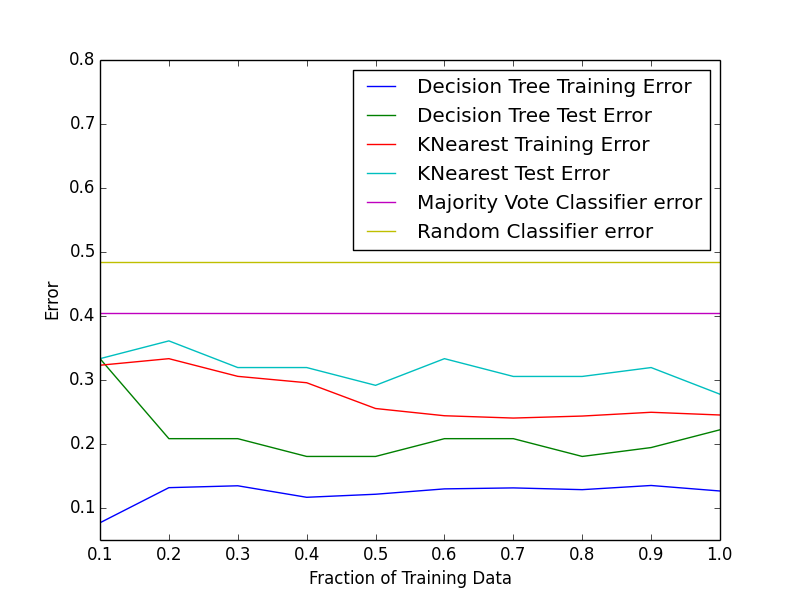
\includegraphics[scale=0.6]{4h.png}
For both the Decision Tree and K-Nearest Neighbors classifier, the error is less than that of the
baseline classifiers we used. For the Decision tree, the training error is quite low, and stays
almost constant for most of the training data, whereas the test data has the lowest error for 
80\% of the training data available. For the K-Nearest Classifiers, the training error decreases,
which means that the algorithm is learning from the training data, however the test data starts
to increase after 50\% of the training data, which could possibly be attributed to overfitting.

\end{enumerate}
\end{document}
